\section{Qualifying compositionality} \label{sec: qualifying}

Now let $\fun{P}\colon \cat{C} \to \cat{D}$ be a \emph{lax} functor of \emph{bicategories}.
This means that, for all triples of objects $X, Y, Z$ in $\cat{C}$, we have two functors
\begin{equation*}
    (\fun{P}-) \Cp (\fun{P}-), \; \fun{P}(- \Cp -)\colon \homset{\cat{C}}{X}{Y} \times \homset{\cat{C}}{Y}{Z} \to \homset{\cat{D}}{\fun{P}X}{\fun{P}Z}
\end{equation*}
connected by a natural transformation, the \emph{laxator} $\varphi\colon (\fun{P}-) \Cp (\fun{P}-) \Rightarrow \fun{P}(- \Cp -)$.\footnote{Technically, the laxators are a family of natural transformations indexed by $X, Y, Z$, but we will leave the indexing implicit.}
As a special case, when $\cat{C}$ and $\cat{D}$ are monoidal categories seen as one-object bicategories, $\fun{P}$ is a lax monoidal functor, and the laxator is a natural transformation $(\fun{P}-) \otimes (\fun{P}-) \Rightarrow \fun{P}(- \otimes -)$.

By Proposition \ref{prop: covariance natural transformation}, we obtain functors $\homset{\cat{C}}{X}{Y} \times \homset{\cat{C}}{Y}{Z} \to \pointed{\catpos}$
sending a pair of morphisms $(f\colon X \to Y, g\colon Y \to Z)$ to the homotopy posets
\begin{equation*}
    \dhom{i}
    {(\slice{\homset{\cat{D}}{\fun{P}X}{\fun{P}Z}}{\fun{P}(f\Cp g)})}
    {\varphi_{f,g}}
\end{equation*}
associated to the component $\varphi_{f,g}$ of the laxator.

In the scenario sketched in the Introduction, the failure of $\varphi_{f,g}$ to be iso is a failure of the ``semantic'' functor $\fun{P}$ to be ``fully compositional'' with respect to the composition $f \Cp g$.
Thus the elements of these homotopy posets may be seen as local \emph{obstructions to compositionality} of $\fun{P}$.
Most interestingly, these obstructions are covariant with respect to the 2-morphisms of $\cat{C}$; thus we can think of ``modifying $f$ and $g$'' by acting on them with a 2-morphism, and see how that affects the obstructions.

\subsection{Open Graphs}\label{subsec: open graphs}
%
%
We apply our framework to a couple of tangible examples.
Open graphs, defined in~\cite{Fong2015}, can be thought of as \emph{graphs with interfaces}. Formally, open graphs are (isomorphism classes of) decorated cospans with decorations in the category $\catgrph$ of graphs and homomorphisms. Intuitively, they are depicted as in the examples below, with \emph{input} vertices on the left and \emph{output} vertices on the right:
%
%
\begin{equation*}
    \scalebox{0.75}{
    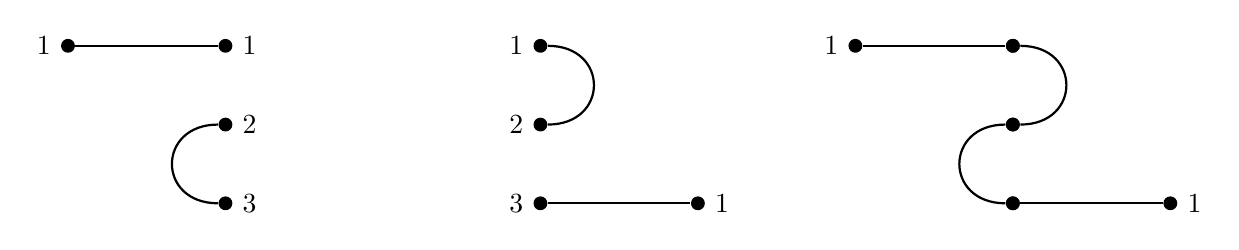
\begin{tikzpicture}
        \begin{scope}[xshift=-2cm]
            \node[circle, fill, minimum size=5pt, inner sep=0pt, label=left:{$1$}] (al1) at (-2,0) {};
            \node[circle, fill, minimum size=5pt, inner sep=0pt, label=right:{$1$}] (ar1) at (0,0) {};
            \node[circle, fill, minimum size=5pt, inner sep=0pt, label=right:{$2$}] (ar2) at (0,-1) {};
            \node[circle, fill, minimum size=5pt, inner sep=0pt, label=right:{$3$}] (ar3) at (0,-2) {};
                \draw[thick] (al1) to (ar1);
                \draw[thick, out=180, in=180, looseness=2] (ar2) to (ar3);
        \end{scope}
        \begin{scope}[xshift=2cm]
            \node[circle, fill, minimum size=5pt, inner sep=0pt, label=right:{$1$}] (br3) at (2,-2) {};
            \node[circle, fill, minimum size=5pt, inner sep=0pt, label=left:{$1$}] (bl1) at (0,0) {};
            \node[circle, fill, minimum size=5pt, inner sep=0pt, label=left:{$2$}] (bl2) at (0,-1) {};
            \node[circle, fill, minimum size=5pt, inner sep=0pt, label=left:{$3$}] (bl3) at (0,-2) {};
                \draw[thick, out=0, in=0, looseness=2] (bl1) to (bl2);
                \draw[thick] (bl3) to (br3);
        \end{scope}
        \begin{scope}[xshift=8cm]
            \begin{scope}[xshift=-0cm]
                \node[circle, fill, minimum size=5pt, inner sep=0pt,label=left:{$1$}] (al1) at (-2,0) {};
                \node[circle, fill, minimum size=5pt, inner sep=0pt] (ar1) at (0,0) {};
                \node[circle, fill, minimum size=5pt, inner sep=0pt] (ar2) at (0,-1) {};
                \node[circle, fill, minimum size=5pt, inner sep=0pt] (ar3) at (0,-2) {};
                    \draw[thick] (al1) to (ar1);
                    \draw[thick, out=180, in=180, looseness=2] (ar2) to (ar3);
            \end{scope}
            \begin{scope}[xshift=0cm]
                \node[circle, fill, minimum size=5pt, inner sep=0pt, label=right:{$1$}] (br3) at (2,-2) {};
                \node[circle, fill, minimum size=5pt, inner sep=0pt] (bl1) at (0,0) {};
                \node[circle, fill, minimum size=5pt, inner sep=0pt] (bl2) at (0,-1) {};
                \node[circle, fill, minimum size=5pt, inner sep=0pt] (bl3) at (0,-2) {};
                    \draw[thick, out=0, in=0, looseness=2] (bl1) to (bl2);
                    \draw[thick] (bl3) to (br3);
            \end{scope}
        \end{scope}
    \end{tikzpicture}}
\end{equation*}
%
Indeed, there is a bicategory $\catopengrph$ that has sets as objects, open graphs as morphisms, and interface-preserving graph homomorphisms as 2-morphisms.
For instance, the first and second open graphs above correspond to morphisms $G\colon \{1\} \to \{1,2,3\}$ and $H\colon \{1,2,3\} \to \{1\}$. 
These morphisms can be composed, resulting in the morphism $G \Cp H\colon \{1\} \to \{1\}$ corresponding to the third open graph in the picture above.

Every graph can be mapped to its \emph{reachability relation}\footnote{Cfr. \cite{lorenz2023causal}, for the similar example of open causal models and causal influence.}: this is a relation on the vertexes of the graph, where two vertexes are considered related iff there is a path between them.
Reachability can be recast as a lax functor $\catopengrph \to \catrel$ to the bicategory of sets, relations, and inclusions of relations, which maps an open graph $G\colon X \to Y$ to the relation $\fun{R}G\colon X \to Y$ defined by
\begin{equation*}
    \text{$\fun{R}G(x, y)$ if and only if there is a path between the input vertex $x$ and the output vertex $y$.}
\end{equation*}
Because $\catrel$ is locally posetal, to define $\fun{R}$ on 2-morphisms it suffices to verify that, if $f\colon G \to G'$ is a graph homomorphism, then $\fun{R}G \subseteq \fun{R}G'$.
The laxators are also uniquely defined.

We can see that this functor is not strong.
In the example above we have that $\fun{R}G \subseteq \{1\} \times \{1,2,3\}$ only contains the pair $(1,1)$, since there are no paths from $1$ to $2$ and from $1$ to $3$ in $G$.
Similarly, $\fun{R}H \subseteq \{1,2,3\} \times \{1\}$ only contains the pair $(3,1)$.
It follows that $\fun{R}G \Cp \fun{R}H\colon \{1\} \to \{1\}$ is the empty relation, but $\fun{R}(G \Cp H)\colon \{1\} \to \{1\}$ is total, so $\fun{R}G \Cp \fun{R}H \subsetneq \fun{R}(G \Cp H)$.

The result is that, if we want to compute the reachability relation of $G \Cp H$ by looking at the reachability relations of $G$ and $H$ separately, we are going to miss something.
This ``compositionality gap'' is tracked by the $\pi_0$ associated to the laxator components $\varphi_{G, H}\colon \fun{R}G \Cp \fun{R}H \subseteq \fun{R}(G \Cp H)$ (because these are all injective, the $\pi_1$ will always be trivial).

In our example, $\dhom{0}{(\slice{\homset{\catrel}{\{1\}}{\{1\}}}{\fun{R}(G\Cp H)})}{\varphi_{G,H}}$ is isomorphic to the poset $(\varnothing < \{(1, 1)\})$ pointed with $\varnothing$, so there is exactly one non-trivial obstruction.
Using covariance, we can think of ``removing the obstruction'' by modifying one or both of the parts $G$ or $H$ with a 2-morphism, that is, with a graph homomorphism.
For example, we can act on $G$ with the homomorphism which identifies the output vertices $1$ and $3$.
The resulting graph $G'$ has $\fun{R}G' = \{(1, 1), (1, 3)\}$, so $\fun{R}G' \Cp \fun{R}H = \fun{R}(G' \Cp H) = \{(1, 1)\}$; correspondingly, we obtain a map of pointed posets from the $\pi_0$ associated to $\varphi_{G, H}$ to the $\pi_0$ associated to $\varphi_{G', H}$, which ``trivialises all obstructions''.
%
%
\subsection{Schr\"odinger Compositionality}\label{subsec: schrodinger compositionality}

The name \emph{Schr\"odinger compositionality} was introduced in \cite{coecke2021compositionality} to refer to the form of compositionality that exists in quantum mechanics, where \emph{non-separable states} are present, to disambiguate it from others.
\footnote{For the purposes of this work, we are leaving out of the present analysis the aspects of Schr\"odinger compositionality regarding the  ``ontological interpretation", originally presented in  \cite{coecke2021compositionality}.}
%One key implication of Schr\"odinger compositionality is that ``a state can be more than its parts''.
In the following, we will focus on the special case of a state that can be ``more than its parts''.
This is arguably what makes composition interesting in quantum mechanics: it makes entanglement possible, which Schr\"odinger described as ``the characteristic trait of quantum mechanics'' \cite{Schrodinger_1935}.
In contrast with the example of open graphs, where the ``compositionality gap'' represents an obstacle to a computation strategy, here it can be seen as a positive feature.
Our approach can be used in both contexts; we will focus on the case study of non-separable states, recasting it as the failure of a lax functor to be strong.

In the context of monoidal categories,
%\footnote{Technically, thoughout the section we implicitly assume that our monoidal categories are strict. The example can easily be reworked for general monoidal categories by introducing unitors where it is suitable.}
a \emph{state} is a morphism $\TensorUnit \to A$, where $\TensorUnit$ is the monoidal unit.
We say that a state $\psi\colon \TensorUnit \to A \otimes B$ is \emph{separable} if there exist states $\psi_A\colon \TensorUnit \to A$ and $\psi_B\colon \TensorUnit \to B$ such that $\psi = \psi_A \otimes \psi_B$.%\footnote{Note that we are referring here to the notion of separability of pure states.}, or, graphically:
%
%
%\begin{equation*}
    %\begin{tikzpicture}
     %   \node[draw,thick,minimum width=2cm, minimum height=0.75cm] (phiAB) at (0,0) {$\psi$};
      %      \draw[thick] ($(phiAB.north) - (0.5,0)$) -- +(0,0.75);
       %     \draw[thick] ($(phiAB.north) + (0.5,0)$) -- +(0,0.75);
       % \node (equals) at (1.75,0) {$=$};
       % \node[draw,thick,minimum width=1cm, minimum height=2] (phiA) at (3,0) {$\psi_{A}$};
       %     \draw[thick] (phiA.north) -- +(0,0.75);
       % \node[draw,thick,minimum width=1cm, minimum height=2] (phiB) at (4.5,0) {$\psi_{B}$};
       %     \draw[thick] (phiB.north) -- +(0,0.75);
    %\end{tikzpicture}
%\end{equation*}
%

%
%
\begin{definition}
    Let $(\cat{C}, \otimes, \TensorUnit)$ be a monoidal category.
    The \emph{state functor} of $\cat{C}$ is the representable functor $\homset{\cat{C}}{\TensorUnit}{-}\colon \cat{C} \to \catset$. 
\end{definition}
%
\begin{proposition}[Laxity of the state functor]\label{prop: state functor lax}
    The state functor lifts to a lax monoidal functor from $(\cat{C}, \otimes, \TensorUnit)$ to $(\catset, \times, \{*\})$, with laxator components
    \begin{align*}
        \varphi_{A,B}\colon \homset{\CategoryC}{\TensorUnit}{A} \times \homset{\CategoryC}{\TensorUnit}{B}
            &\rightarrow 
            \homset{\CategoryC}{\TensorUnit}{A \otimes B}\\
        (\psi_A, \psi_B) 
            &\mapsto
            \psi_A \otimes \psi_B.
    \end{align*}
\end{proposition}
%
%
Recall that a monoidal category is \emph{semicartesian} if its monoidal unit is terminal.
The following result is a consequence of the general fact that a functor from a semicartesian to a cartesian monoidal category has a canonical oplax monoidal structure.
%
%
\begin{proposition}[Oplaxity of the state functor]\label{prop: state functor oplax}
    Let $(\cat{C}, \otimes, \Term)$ be a semicartesian category.
    Then the state functor lifts to an oplax monoidal functor from $(\cat{C}, \otimes, \Term)$ to $(\catset, \times, \{*\})$.
\end{proposition}
%
Clearly, there are cases where the state functor is not just lax or oplax, but strong.
The following result captures the well-known fact that in a cartesian monoidal category every state is separable.
%
\begin{proposition}[Strongness of the state functor]\label{prop: state functor strong}
    If $(\CategoryC, \times, \Term)$ is cartesian, then the state functor is strong monoidal.
\end{proposition}

Having turned Schr\"odinger compositionality into a question about (op)laxity of a functor, we can put our framework to good work.
By \autoref{prop: covariance natural transformation}, we have functors $\cat{C} \times \cat{C} \to \pointed{\catpos}$ sending pairs of objects $(A, B)$ of $\cat{C}$ to the homotopy posets 
\begin{equation} \label{eq: state_dhom }
    \dhom{i}{(\slice{\Set}{\homset{\cat{C}}{I}{A \otimes B}})}{\varphi_{A, B}}, \quad i \in \{ 0, 1 \}.
\end{equation}
Using the description of homotopy posets for slices of $\Set$ from \autoref{sec: obstructions}, we see that
\begin{itemize}
    \item minimal obstructions in $\pi_0$ are in bijection with non-separable states of $A \otimes B$,
    \item minimal obstructions in $\pi_1$ are in bijection with pairs of pairs of states $((\psi_A, \psi_B), (\chi_A, \chi_B))$ such that $\psi_A \otimes \psi_B = \chi_A \otimes \chi_B$.
\end{itemize}
For example, in $(\lcat{Vect}_\mathbb{C}, \otimes, \mathbb{C})$, the monoidal category of complex vector spaces with their tensor product, whenever $A$ and $B$ are at least 2-dimensional, we have instances of both:
\begin{itemize}
    \item the state $1 \mapsto \begin{pmatrix}1 \\ 0\end{pmatrix} \otimes \begin{pmatrix}1 \\ 0\end{pmatrix} + \begin{pmatrix}0 \\ 1\end{pmatrix} \otimes \begin{pmatrix}0 \\ 1\end{pmatrix}$ of $\mathbb{C}^2 \otimes \mathbb{C}^2$ is non-separable,
    \item given any pair of states $(\psi_A, \psi_B)$ and any non-zero $\lambda \in \mathbb{C}$, the pair $(\chi_A, \chi_B) \eqdef (\lambda \psi_A, \invrs{\lambda} \psi_B)$ satisfies $\psi_A \otimes \psi_B = \chi_A \otimes \chi_B$.
\end{itemize}
We can derive a few simple, immediate consequences from the covariance of (\ref{eq: state_dhom }) in the pair $(A, B)$.
\begin{enumerate}
    \item Given morphisms $f\colon A \to A'$, $g\colon B \to B'$, the induced maps of posets preserve the basepoint, that is, map ``non-obstructions'' to ``non-obstructions''.
    In this case, this implies that \emph{it is not possible to entangle a separable state by local actions}, that is, by applying morphisms on $A$ and $B$ separately.
    \item On the other hand, it is, in principle, possible for the induced maps to send non-trivial obstructions to the basepoint.
    For example, in complex vector spaces, acting on $A$ or $B$ with a rank-1 linear map always has a separating effect.
\end{enumerate}
